%==============================================================================
%  Business Intelligence (IT5315E) - Group Project Report
%  Real-Time Payment Fraud Detection for an E-Commerce Platform
%
%  Compiles with pdfLaTeX (default on Overleaf) OR XeLaTeX/LuaLaTeX.
%  Figures live in ./figures/  (copied from docs/figures/paysim/).
%  Recommended build:  latexmk -pdf main.tex     (run twice for the ToC/refs)
%==============================================================================
\documentclass[11pt,a4paper]{report}

%------------------------------------------------------------------ encoding/fonts
\usepackage{iftex}
\ifPDFTeX
  \usepackage[utf8]{inputenc}   % UTF-8 source (Vietnamese names)
  \usepackage{lmodern}
  \usepackage[T5]{fontenc}      % T5 = Vietnamese encoding (superset of Latin for English)
\else
  \usepackage{fontspec}         % XeLaTeX/LuaLaTeX: use a system Unicode font
\fi
\usepackage[english]{babel}

%------------------------------------------------------------------ layout
\usepackage[a4paper,margin=2.4cm]{geometry}
\usepackage{graphicx}
\usepackage{booktabs}
\usepackage{longtable}
\usepackage{array}
\usepackage{multirow}
\usepackage{makecell}
\usepackage{tabularx}
\usepackage{xcolor}
\usepackage{caption}
\usepackage{subcaption}
\usepackage{amsmath,amssymb}
\usepackage{enumitem}
\usepackage{fancyhdr}
\usepackage{titlesec}
\usepackage[most]{tcolorbox}
\usepackage[hidelinks]{hyperref}

%------------------------------------------------------------------ theme colours
\definecolor{brandteal}{RGB}{20,86,102}
\definecolor{brandaccent}{RGB}{198,52,72}
\definecolor{lightgray}{RGB}{244,246,247}
\definecolor{midgray}{RGB}{110,120,124}

\hypersetup{
  colorlinks=true,
  linkcolor=brandteal,
  citecolor=brandteal,
  urlcolor=brandaccent,
  pdftitle={Real-Time Payment Fraud Detection for an E-Commerce Platform},
  pdfauthor={BI Group Project - HUST}
}

%------------------------------------------------------------------ section styling
\titleformat{\chapter}[display]
  {\normalfont\huge\bfseries\color{brandteal}}
  {\chaptertitlename\ \thechapter}{16pt}{\Huge}
\titleformat{\section}
  {\normalfont\Large\bfseries\color{brandteal}}{\thesection}{1em}{}
\titleformat{\subsection}
  {\normalfont\large\bfseries\color{brandteal!85!black}}{\thesubsection}{1em}{}

\captionsetup{font=small,labelfont={bf,color=brandteal}}

%------------------------------------------------------------------ header/footer
\pagestyle{fancy}
\fancyhf{}
\renewcommand{\headrulewidth}{0.4pt}
\fancyhead[L]{\small\color{midgray}Business Intelligence (IT5315E)}
\fancyhead[R]{\small\color{midgray}E-Commerce Fraud Detection}
\fancyfoot[C]{\thepage}

%------------------------------------------------------------------ helper boxes
\newtcolorbox{keybox}[1][]{
  colback=lightgray, colframe=brandteal, boxrule=0.8pt, arc=2pt,
  left=8pt,right=8pt,top=6pt,bottom=6pt, #1}
\newtcolorbox{warnbox}[1][]{
  colback=brandaccent!6, colframe=brandaccent, boxrule=0.8pt, arc=2pt,
  left=8pt,right=8pt,top=6pt,bottom=6pt, #1}
\newtcolorbox{todobox}[1][]{
  colback=yellow!8, colframe=orange!80!black, boxrule=0.8pt, arc=2pt,
  left=8pt,right=8pt,top=6pt,bottom=6pt, #1}

\newcommand{\code}[1]{\texttt{\small #1}}
\newcolumntype{Y}{>{\raggedright\arraybackslash}X}
\emergencystretch=3em   % avoid overfull lines from long \texttt tokens
\hyphenpenalty=1000

%==============================================================================
\begin{document}

%------------------------------------------------------------------ TITLE PAGE
\begin{titlepage}
\centering
\vspace*{0.4cm}

\includegraphics[width=0.30\textwidth]{figures/hust-full.png}\par
\vspace{0.5cm}
{\color{midgray}\large HANOI UNIVERSITY OF SCIENCE AND TECHNOLOGY\par}
{\color{midgray}\large School of Information and Communications Technology\par}
{\color{midgray}\normalsize Master's Programme in Data Science\par}
\vspace{0.4cm}
{\color{brandteal}\rule{\textwidth}{1.2pt}}\par
\vspace{1.1cm}

{\color{midgray}\normalsize BUSINESS INTELLIGENCE - GROUP PROJECT REPORT\par}
\vspace{0.3cm}
{\Huge\bfseries\color{brandteal} Real-Time Payment Fraud Detection\\[6pt] for an E-Commerce Platform\par}
\vspace{0.5cm}
{\large\itshape An End-to-End Analytics Project:\\ From Raw Data to a Monitored, Deployed Model\par}
\vspace{0.9cm}
{\color{brandteal}\rule{0.5\textwidth}{0.8pt}}\par
\vspace{0.9cm}

\begin{tabular}{@{}rl@{}}
\textbf{Course} & Business Intelligence (IT5315E)\\[3pt]
\textbf{Instructor} & Assoc. Prof. Bùi Quốc Trung\\[3pt]
\textbf{Domain} & E-Commerce - Payment Risk \& Trust\\[3pt]
\textbf{Report scope} & Modules 1–8 (complete end-to-end lifecycle)\\
\end{tabular}

\vspace{1.0cm}
{\large\bfseries\color{brandteal} Team Members\par}
\vspace{0.2cm}
\begin{tabular}{@{}ll@{}}
\toprule
\textbf{Full name} & \textbf{Student ID}\\
\midrule
Lương Minh Dương    & 20251038M\\
Trần Lê Phương Thảo  & 20251186M\\
Hoàng Minh Hoàng     & 20252561M\\
Ngô Việt Anh         & 20252570M\\
Phạm Tuấn Kiệt       & 20252751M\\
Nguyễn Như Thái      & 20252270M\\
\bottomrule
\end{tabular}

\vfill
{\color{midgray} Hanoi, July 2026\par}
\end{titlepage}

%------------------------------------------------------------------ ABSTRACT
\chapter*{Abstract}
\addcontentsline{toc}{chapter}{Abstract}
\thispagestyle{fancy}

This report documents an end-to-end business-intelligence product that scores online
payment transactions for fraud risk in real time. Acting as the risk-analytics function
of an e-commerce platform, we answer a concrete business question: \emph{which incoming
transactions are likely to be fraudulent, and how should the platform balance blocking
fraud against approving legitimate orders without unnecessary friction?}

We combine the public \textbf{PaySim} transaction dataset (6{,}362{,}620 records, fraud
prevalence 0.129\%) with a purpose-built \textbf{synthetic contextual layer} - identity,
device, geolocation, and behavioural risk signals generated in Python with Faker plus
custom business logic, each field documented in a full data dictionary. The pipeline
proceeds through exploratory data analysis, conservative cleaning, leakage-aware feature
engineering with explicit class-imbalance handling, and a comparative model-development
stage that selects an operating threshold from a business cost function.

The central methodological contribution is a strict separation between \emph{leaky} and
\emph{deployable} features. PaySim's post-transaction balance fields near-deterministically
encode the label but are unknown at authorization time; models trained on them reach an
artificial AUC-PR of $\approx 1.0$. We exclude them from deployment and instead ship a
model trained only on authorization-time signals. The deployable model - \textbf{XGBoost}
on the 44-feature \code{realistic} group - achieves a held-out test \textbf{AUC-PR of
0.907}, \textbf{ROC-AUC of 0.999}, \textbf{recall of 98.1\%}, and avoids \textbf{99.9\%}
of fraud loss while flagging only \textbf{2.4\%} of transactions.

The model is then productionised as a complete analytics product: a \textbf{three-model
ensemble} (Logistic Regression, Random Forest, XGBoost) served behind a FastAPI
\code{/score} endpoint that returns each model's verdict plus a \emph{max-risk} aggregate
(\code{block > review > allow}); an eight-page Streamlit analyst application (executive
overview, segment analytics, review queue with reason codes, model evaluation, cost/ROI,
live feed, monitoring, and an API tester) deployable to a single free-tier port via an
embedded API; and a monitoring layer that tracks per-feature and per-model
Population-Stability-Index (PSI) drift, fires a retraining trigger at PSI $\ge 0.25$,
supports in-app retraining, and emits webhook alerts. This report documents the full
lifecycle across all eight modules.

\vspace{0.3cm}
\noindent\textbf{Keywords:} fraud detection, class imbalance, XGBoost, cost-sensitive
threshold, data leakage, PaySim, synthetic data, AUC-PR.

%------------------------------------------------------------------ TOC
\tableofcontents
\thispagestyle{fancy}

%==============================================================================
\chapter{Introduction and Business Understanding}
\label{ch:intro}
%==============================================================================

\section{Project context and business question}

E-commerce platforms process thousands of transactions per minute. Even a fraud rate well
under 5\% translates into significant financial loss and eroded customer trust. This
project asks the team to build, deploy, and monitor a classifier that flags high-risk
transactions in real time, mirroring the full lifecycle of an analytics product in
industry. The guiding business question is:

\begin{keybox}
\textit{``Which incoming transactions are likely to be fraudulent, and how should the
platform balance blocking fraud against approving legitimate orders without unnecessary
friction?''}
\end{keybox}

The trade-off is inherently three-sided:
\begin{itemize}[nosep,leftmargin=1.4em]
  \item \textbf{Missed fraud} (false negatives) causes direct financial loss, roughly
        proportional to the transaction amount.
  \item \textbf{False alarms} (false positives) create customer friction, potential churn,
        and manual-review labour.
  \item \textbf{Manual-review capacity} is finite, so every flag consumes a scarce
        resource.
\end{itemize}

A good policy therefore cannot be chosen by accuracy alone; it must be chosen against a
\emph{cost model} that prices these outcomes in a common currency. This principle drives
our metric choice (AUC-PR and a cost-based objective rather than accuracy) and our
operating-threshold selection (Section~\ref{sec:cost}).

\section{Key performance indicators (KPIs)}

We define three KPIs that connect the model directly to business value.

\begin{table}[h]
\centering
\small
\begin{tabularx}{\textwidth}{@{}l l Y@{}}
\toprule
\textbf{KPI} & \textbf{Formula} & \textbf{Business meaning}\\
\midrule
Fraud rate (prevalence) & $N_{\text{fraud}} / N_{\text{txn}}$ &
Base rate the model must handle. PaySim: $8{,}213 / 6{,}362{,}620 = 0.129\%$.\\
\addlinespace
False-positive rate & $FP / (FP+TN)$ &
Share of legitimate transactions wrongly flagged. Lower $\Rightarrow$ less friction.\\
\addlinespace
Financial loss avoided & $\dfrac{\sum \text{amount}(TP)}{\sum \text{amount}(\text{all fraud})}$ &
Share of fraudulent money intercepted before loss.\\
\bottomrule
\end{tabularx}
\caption{Business KPIs used throughout the project.}
\label{tab:kpi}
\end{table}

\noindent The total exposed fraud amount in PaySim is \textbf{12{,}056{,}415{,}427.84}
currency units; ``loss avoided'' is measured against this denominator.

\section{Cost model overview}
\label{sec:costoverview}

Threshold selection (Module 5) minimises an \emph{expected cost} that turns the three-sided
trade-off into a single scalar:
\begin{equation}
\label{eq:cost}
\text{Cost} =
\underbrace{c_{FN}\!\!\sum_{i\in FN}\!\text{amount}_i}_{\text{missed fraud}}
+\underbrace{c_{FP}\cdot|FP|}_{\text{friction}}
+\underbrace{c_{MR}\cdot|\text{flagged}|}_{\text{review labour}} .
\end{equation}
The coefficients $c_{FN}, c_{FP}, c_{MR}$ are business assumptions kept in
\code{src/config.py} so that threshold selection and the report never drift apart. Their
derivation, current values, and a sensitivity discussion are given in
Section~\ref{sec:cost}.

\section{Team and role distribution}

The project follows the suggested five-role structure; with a six-person team the
report/presentation duty is shared. Table~\ref{tab:roles} shows the proposed distribution
(adjustable by the team).

\begin{table}[h]
\centering
\small
\begin{tabularx}{\textwidth}{@{}l l Y@{}}
\toprule
\textbf{Member} & \textbf{Role} & \textbf{Primary responsibilities}\\
\midrule
Lương Minh Dương   & Data Engineer            & Synthetic data generation, data dictionary, cleaning\\
Trần Lê Phương Thảo & Data Analyst             & Exploratory data analysis, fraud-pattern visualization\\
Hoàng Minh Hoàng    & ML Engineer (Modeling)   & Feature engineering, classifier development\\
Ngô Việt Anh        & ML Engineer (Evaluation) & Imbalance handling, threshold and cost-based evaluation\\
Phạm Tuấn Kiệt      & MLOps Lead               & Deployment (API + review queue), drift monitoring\\
Nguyễn Như Thái     & MLOps / Reporting        & Monitoring support, final report and presentation\\
\bottomrule
\end{tabularx}
\caption{Proposed team roles (adapted from the project brief; to be confirmed by the team).}
\label{tab:roles}
\end{table}

\section{Repository and reproducibility}

All code is authored by the team (no AutoML platforms). The pipeline is fully scripted and
reproducible from a single fixed seed (\code{SEED=42}); Table~\ref{tab:modmap} maps each
module to its source. Heavy artefacts (raw CSV, processed parquet, model bundles) are
regenerated locally rather than committed.

\begin{table}[h]
\centering
\small
\begin{tabularx}{\textwidth}{@{}c l Y@{}}
\toprule
\textbf{\#} & \textbf{Module} & \textbf{Source files}\\
\midrule
1 & Business understanding \& data generation & \code{src/synth\_context.py}, \code{src/build\_dataset.py}, \code{docs/data\_dictionary.md}\\
2 & Exploratory data analysis & \code{src/eda.py}\\
3 & Data cleaning & \code{src/cleaning.py}\\
4 & Feature engineering & \code{src/features.py}, \code{src/imbalance.py}\\
5 & Model development \& ensemble & \code{src/train\_validate.py}, \code{src/ensemble.py}, \code{src/infer.py}\\
6 & Deployment & \code{api/main.py}, \code{app/*.py} (8-page app), \code{app/embedded\_api.py}, \code{src/costs.py}, \code{src/reasons.py}\\
7 & Monitoring & \code{monitoring/drift.py}, \code{app/monitoring\_view.py}, \code{src/retrain.py}, \code{src/alerting.py}\\
8 & Report \& presentation & this document\\
\bottomrule
\end{tabularx}
\caption{Module-to-file map. Steps 1–5 run together via \code{./train.sh full}.}
\label{tab:modmap}
\end{table}

%==============================================================================
\chapter{Data Sources and Synthetic Data Generation (Module 1)}
\label{ch:m1}
%==============================================================================

\section{Base dataset: PaySim}

The required base is the Kaggle \emph{Online Payments Fraud Detection Dataset}~\cite{kaggle}
(dataset id \code{rupakroy/} \code{online-payments-fraud-detection-dataset}), a PaySim
simulation of mobile money transactions. Key structural facts, confirmed on the full file:

\begin{itemize}[nosep,leftmargin=1.4em]
  \item \textbf{6{,}362{,}620} transactions over \textbf{743} hourly steps ($\approx$30 days).
  \item \textbf{8{,}213} frauds - a prevalence of \textbf{0.129\%} (severe imbalance).
  \item Fraud occurs \emph{only} in \code{TRANSFER} and \code{CASH\_OUT} transactions.
  \item Eleven base columns: \code{step}, \code{type}, \code{amount},
        \code{nameOrig}/\code{nameDest}, four balance fields, \code{isFraud} (target),
        and PaySim's own rule flag \code{isFlaggedFraud}.
\end{itemize}

PaySim provides transactions, balances, and labels but \emph{no} e-commerce risk context -
no customer tenure, device fingerprint, geolocation, address mismatch, or failed-payment
history. The project brief therefore requires a synthetic contextual extension.

\section{Why and how we generate synthetic context}

We add a transparent synthetic layer with \emph{overlapping} fraud/legitimate distributions,
so that no synthetic field perfectly separates the classes. This keeps the task realistic
(the synthetic signals \emph{support} detection rather than trivially solving it). The
generator (\code{src/synth\_context.py}) is organised into three layers:

\begin{itemize}[nosep,leftmargin=1.4em]
  \item \textbf{L1 - Identity} (display/context only): \code{customer\_id},
        \code{customer\_name}, \code{email}, \code{billing\_city}. A fixed pool of
        200{,}000 Faker identities is used because the real \code{nameOrig} is almost
        always single-use.
  \item \textbf{L2 - Account risk}: \code{account\_age\_days} (lognormal),
        \code{high\_risk\_country} / \code{billing\_country}, \code{is\_disposable\_email}.
  \item \textbf{L3 - Transaction / device / time risk}: \code{is\_new\_device},
        \code{shipping\_billing\_mismatch}, \code{num\_failed\_payment\_attempts} (Poisson),
        \code{ip\_billing\_distance\_km} (Haversine from home to a simulated IP),
        \code{browser}, \code{device\_os}, time features, and illustrative account velocity.
\end{itemize}

\subsection{The reveal/noise softening mechanism}

Rather than drawing a risk flag directly from the label (which would create perfect
leakage), each fraud-conditioned field is generated through an \emph{effective risk mask}:
\begin{equation}
\text{risky}_i = \big(\text{isFraud}_i \wedge U_i < r\big) \;\vee\; \big(\neg\text{isFraud}_i \wedge V_i < n\big),
\end{equation}
with \emph{reveal rate} $r=0.55$ and \emph{legit noise} $n=0.04$ ($U_i,V_i \sim \text{Uniform}(0,1)$).
Only when $\text{risky}_i$ is true does the field draw from its ``fraud'' distribution.
Consequently many frauds look benign and some legitimate rows look risky - exactly the
ambiguity a real detector faces. Table~\ref{tab:genparams} lists the parameters.

\begin{table}[h]
\centering
\small
\begin{tabularx}{\textwidth}{@{}l l l Y@{}}
\toprule
\textbf{Field} & \textbf{Legit} & \textbf{Fraud} & \textbf{Distribution / note}\\
\midrule
\code{account\_age\_days}            & $(6.0, 0.9)$ & $(5.0, 1.0)$ & Lognormal $(\mu,\sigma)$, clipped 1–3650 days\\
\code{high\_risk\_country}           & 0.06 & 0.28 & Bernoulli; high-risk = NG/RU/CN/ID\\
\code{is\_disposable\_email}         & 0.04 & 0.22 & Bernoulli; disposable vs.\ common domain\\
\code{is\_new\_device}               & 0.15 & 0.50 & Bernoulli\\
\code{shipping\_billing\_mismatch}   & 0.08 & 0.42 & Bernoulli\\
\code{num\_failed\_payment\_attempts}& $\lambda=0.30$ & $\lambda=1.40$ & Poisson\\
\code{ip\_billing\_distance\_km}     & $(0.2,1.0)$ & $(1.4,1.1)$ & Lognormal offset (deg) $\to$ Haversine km\\
\bottomrule
\end{tabularx}
\caption{Synthetic generation parameters. Reveal rate $r=0.55$, legit noise $n=0.04$,
$n_{\text{customers}}=200{,}000$, \code{SEED}=42.}
\label{tab:genparams}
\end{table}

\section{Data dictionary}

Every synthetically generated field is documented with column name, data type, unit, valid
range, and generation logic, as required by the brief. Table~\ref{tab:datadict_base} covers
the base PaySim columns and Table~\ref{tab:datadict_synth} the synthetic layer.

\begin{table}[h]
\centering
\footnotesize
\begin{tabularx}{\textwidth}{@{}l l l l Y@{}}
\toprule
\textbf{Column} & \textbf{Type} & \textbf{Unit} & \textbf{Range} & \textbf{Description}\\
\midrule
\code{step} & int & hours & 1..743 & Simulation time; one step $=$ one hour.\\
\code{type} & cat & -- & 5 types & \code{PAYMENT/TRANSFER/CASH\_OUT/CASH\_IN/DEBIT}; fraud only in TRANSFER \& CASH\_OUT.\\
\code{amount} & float & currency & $\ge 0$ & Transaction amount; proxy for fraud loss.\\
\code{nameOrig} & string & -- & C\#\#\# & Origin customer id; almost always single-use.\\
\code{oldbalanceOrg} & float & currency & $\ge 0$ & Origin balance before.\\
\code{newbalanceOrig} & float & currency & $\ge 0$ & Origin balance after (\emph{post-transaction}).\\
\code{nameDest} & string & -- & C/M\#\#\# & Destination account; reused accounts are mule candidates.\\
\code{oldbalanceDest} & float & currency & $\ge 0$ & Destination balance before.\\
\code{newbalanceDest} & float & currency & $\ge 0$ & Destination balance after (\emph{post-transaction}).\\
\code{isFraud} & int & flag & \{0,1\} & \textbf{Target label}.\\
\code{isFlaggedFraud} & int & flag & \{0,1\} & PaySim's built-in rule flag for very large transfers.\\
\bottomrule
\end{tabularx}
\caption{Data dictionary - base PaySim columns.}
\label{tab:datadict_base}
\end{table}

{\footnotesize
\setlength{\tabcolsep}{4pt}
\begin{longtable}{@{}p{4.6cm} p{1.6cm} p{2.3cm} p{6.3cm}@{}}
\caption{Data dictionary - synthetic contextual layer (Module 1). Fields are grouped by risk
layer; a field is \emph{fraud-conditioned} (softened via the reveal/noise mask) wherever its
logic lists distinct legit/fraud parameters.}
\label{tab:datadict_synth}\\
\toprule
\textbf{Column} & \textbf{Type / unit} & \textbf{Range} & \textbf{Generation logic / business assumption}\\
\midrule
\endfirsthead
\multicolumn{4}{@{}l}{\small\itshape Table~\ref{tab:datadict_synth} continued}\\
\toprule
\textbf{Column} & \textbf{Type / unit} & \textbf{Range} & \textbf{Generation logic / business assumption}\\
\midrule
\endhead
\midrule \multicolumn{4}{r@{}}{\small\itshape continued on next page}\\
\endfoot
\bottomrule
\endlastfoot
\multicolumn{4}{@{}l}{\textbf{\color{brandteal}L1 - Identity (display / context only)}}\\
\texttt{customer\_id} & string & U0..U199999 & Assigned from a fixed synthetic customer pool because real \texttt{nameOrig} is single-use.\\
\texttt{customer\_name} & string & Faker name & Faker name for review-queue / demo display only; not a model feature.\\
\texttt{email} & string & handle@domain & Faker handle + common or disposable domain per \texttt{is\_disposable\_email}.\\
\texttt{billing\_city} & string & Faker city & Faker city for analyst-facing context.\\
\addlinespace
\multicolumn{4}{@{}l}{\textbf{\color{brandteal}L2 - Account risk}}\\
\texttt{account\_age\_days} & int / days & 1..3650 & Lognormal days; legit $(6.0,0.9)$, fraud $(5.0,1.0)$, via reveal/noise mask.\\
\texttt{billing\_country} & cat & 12 ISO codes & High-risk = NG/RU/CN/ID; selected by \texttt{high\_risk\_country}.\\
\texttt{high\_risk\_country} & int / flag & \{0,1\} & Bernoulli; legit 0.06, fraud 0.28.\\
\texttt{is\_disposable\_email} & int / flag & \{0,1\} & Bernoulli; legit 0.04, fraud 0.22.\\
\addlinespace
\multicolumn{4}{@{}l}{\textbf{\color{brandteal}L3 - Transaction / device / time risk}}\\
\texttt{is\_new\_device} & int / flag & \{0,1\} & Bernoulli; legit 0.15, fraud 0.50.\\
\texttt{shipping\_billing\_mismatch} & int / flag & \{0,1\} & Bernoulli; legit 0.08, fraud 0.42.\\
\texttt{num\_failed\_payment\_attempts} & int / count & $\ge 0$ & Poisson; legit $\lambda{=}0.3$, fraud $\lambda{=}1.4$.\\
\texttt{browser} & cat & 6 values & Uniform draw from common browsers.\\
\texttt{device\_os} & cat & 5 values & Uniform draw from common OSes.\\
\texttt{device\_id} & string & D\#\#\# & Random device fingerprint id.\\
\texttt{ip\_billing\_distance\_km} & float / km & $\ge 0$ & Haversine home$\to$IP; offset deg legit $(0.2,1.0)$, fraud $(1.4,1.1)$.\\
\texttt{hour\_of\_day} & int / hour & 0..23 & Derived: \texttt{step} mod 24.\\
\texttt{day\_index} & int / day & 0..30 & Derived: \texttt{step} $//$ 24.\\
\texttt{is\_night} & int / flag & \{0,1\} & Derived: 1 when hour $\in$ 0..5.\\
\texttt{account\_txn\_total} & int / count & $\ge 1$ & Total synthetic-customer transactions (illustrative).\\
\texttt{account\_txn\_index} & int / count & $\ge 0$ & 0-based transaction order per synthetic customer.\\
\texttt{time\_since\_last\_hours} & int / hours & $-1$ or $\ge 0$ & Hours since previous synthetic-customer txn ($-1$ if first).\\
\texttt{txn\_count\_last\_24h} & int / count & $\ge 0$ & Prior synthetic-customer txns in trailing 24h.\\
\end{longtable}}

\section{Design notes and honest limitations}

\begin{itemize}[nosep,leftmargin=1.4em]
  \item Faker identity columns are analyst-facing context, \emph{not} real PII, and are
        dropped before modelling.
  \item Because real \code{nameOrig} is single-use, synthetic per-customer velocity is
        \emph{illustrative}; the genuinely useful account-level signal comes from repeated
        \code{nameDest} (mule) aggregation, which we build causally in Module 4.
  \item PaySim's post-transaction balance fields are extremely predictive. We flag this
        early (Section~\ref{sec:balance}) and treat balance-reconciliation features as a
        separate ``leaky'' track that is \emph{excluded} from the deployed model.
\end{itemize}

%==============================================================================
\chapter{Exploratory Data Analysis (Module 2)}
\label{ch:m2}
%==============================================================================

EDA is computed by \code{src/eda.py}. Raw-sensitive sections (type, amount, balance,
\code{nameDest} reuse) use the full 6.36M-row CSV to avoid sampling artefacts; some
context sections use a stratified processed sample ($\approx$954k rows) that preserves the
natural fraud rate.

\section{Class imbalance}

The dataset is severely imbalanced: 6{,}354{,}407 legitimate vs.\ 8{,}213 fraudulent rows
(Figure~\ref{fig:imbalance}). This 774:1 ratio dictates every downstream choice - we
prefer AUC-PR over accuracy, use class weights, and select the threshold from a cost
function rather than the default 0.5.

\begin{figure}[h]
\centering

\includegraphics[width=0.52\textwidth]{figures/01_class_imbalance.png}
\caption{Class imbalance (log scale): fraud is only 0.129\% of transactions.}
\label{fig:imbalance}
\end{figure}

\section{Fraud by transaction type}

Fraud is structurally confined to two transaction types (Figure~\ref{fig:bytype},
Table~\ref{tab:bytype}): \code{TRANSFER} (0.77\% fraud rate) and \code{CASH\_OUT}
(0.18\%). \code{PAYMENT}, \code{CASH\_IN}, and \code{DEBIT} contain \emph{no} fraud. This
is the single strongest structural prior in the data and motivates the \code{is\_transfer}
/ \code{is\_cash\_out} indicator features.

\begin{minipage}{0.5\textwidth}
\centering

\includegraphics[width=\textwidth]{figures/02_fraud_by_type.png}
\captionof{figure}{Fraud rate by transaction type.}
\label{fig:bytype}
\end{minipage}\hfill
\begin{minipage}{0.47\textwidth}
\centering
\small
\begin{tabular}{@{}lrr@{}}
\toprule
\textbf{Type} & \textbf{Frauds} & \textbf{Rate \%}\\
\midrule
TRANSFER & 4{,}097 & 0.769\\
CASH\_OUT & 4{,}116 & 0.184\\
CASH\_IN & 0 & 0.000\\
DEBIT & 0 & 0.000\\
PAYMENT & 0 & 0.000\\
\bottomrule
\end{tabular}
\captionof{table}{Fraud counts and rates by type.}
\label{tab:bytype}
\end{minipage}

\section{Amount distribution and outliers}

Transaction amounts are heavy-tailed: median $\approx 74{,}872$, the 99.9th percentile
$\approx 8.96$M, and a maximum of $92{,}445{,}516$. Fraudulent transactions skew towards
larger amounts (Figure~\ref{fig:amount}). Binning amount into deciles
(Figure~\ref{fig:decile}) shows the fraud rate rising sharply in the top decile
(0.69\%) - an order of magnitude above the low deciles ($\approx$0.02\%). This motivates
\code{log\_amount} and confirms that amount is a genuine (if weak on its own) signal.

\begin{figure}[h]
\centering
\begin{subfigure}{0.48\textwidth}
  
\includegraphics[width=\textwidth]{figures/03_amount_by_class.png}
  \caption{Amount density by class ($\log 1p$).}
\end{subfigure}\hfill
\begin{subfigure}{0.48\textwidth}
  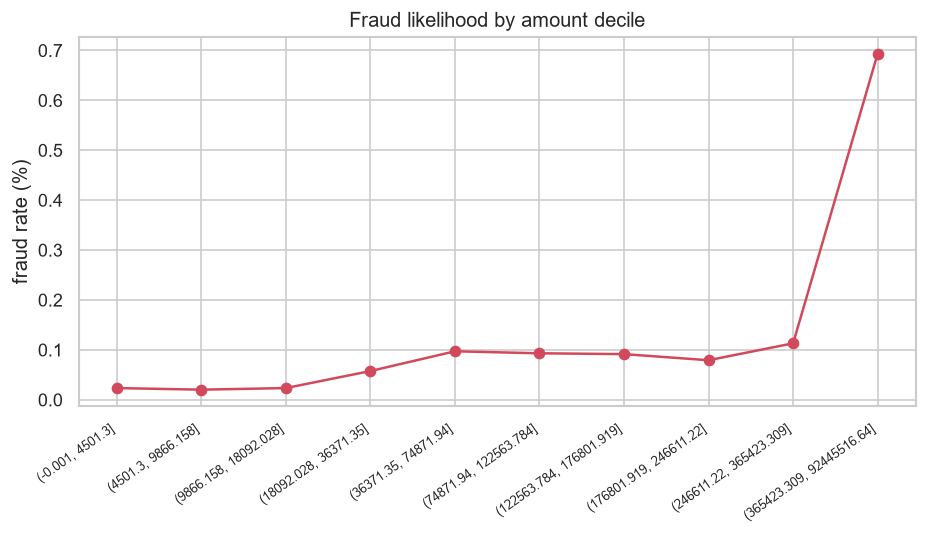
\includegraphics[width=\textwidth]{figures/04_amount_decile_fraud_rate.png}
  \caption{Fraud rate by amount decile.}
  \label{fig:decile}
\end{subfigure}
\caption{Transaction amount vs.\ fraud likelihood. Fraud concentrates in large amounts.}
\label{fig:amount}
\end{figure}

\section{Temporal patterns}

Fraud has a striking diurnal signature (Figure~\ref{fig:time}, left): the fraud rate peaks
at roughly \textbf{22\%} in the 04:00–05:00 window and is negligible during the day. The derived
\code{is\_night} flag captures this - night transactions carry a 1.77\% fraud rate versus
0.10\% otherwise. The per-day panel (right) shows a spike on the final simulation day; this
is a low-volume simulation quirk (a handful of rows) rather than a real pattern, and we
treat it as such.

\begin{figure}[h]
\centering
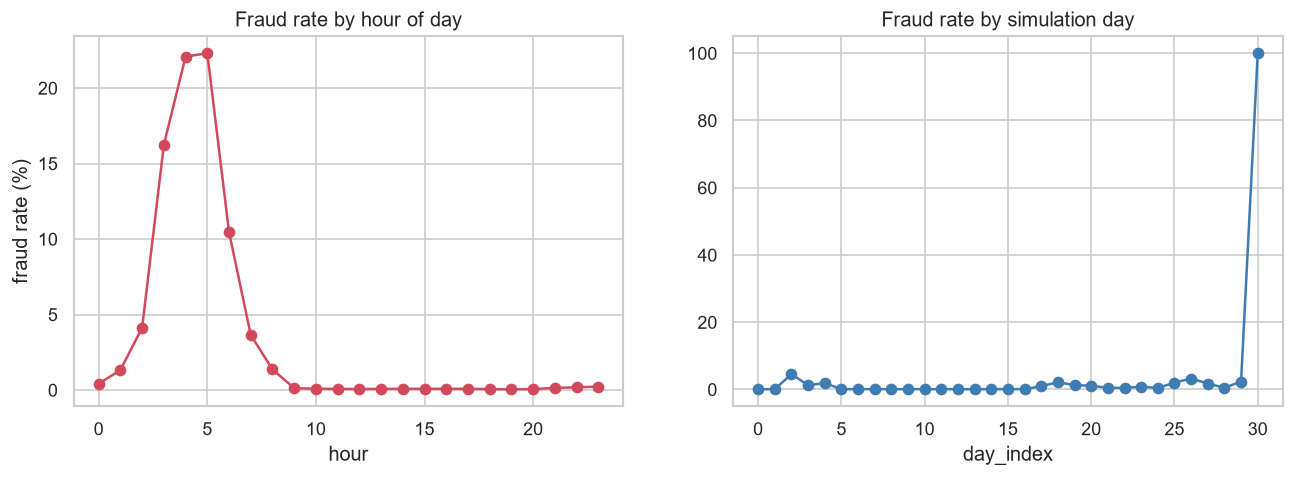
\includegraphics[width=0.92\textwidth]{figures/05_time_windows.png}
\caption{Fraud rate by hour of day (left) and by simulation day (right).}
\label{fig:time}
\end{figure}

\section{Synthetic risk flags}

The synthetic risk flags behave as designed (Figure~\ref{fig:flags}, Table~\ref{tab:flags}):
each of the account/device/context flags roughly doubles-to-triples the fraud rate when set,
while the temporal \code{is\_night} flag lifts it far more - from 0.10\% to 1.77\%
($\approx$17$\times$). None is deterministic, however - the overlap engineered via the
reveal/noise mechanism is visible and intended.

\begin{minipage}{0.55\textwidth}
\centering
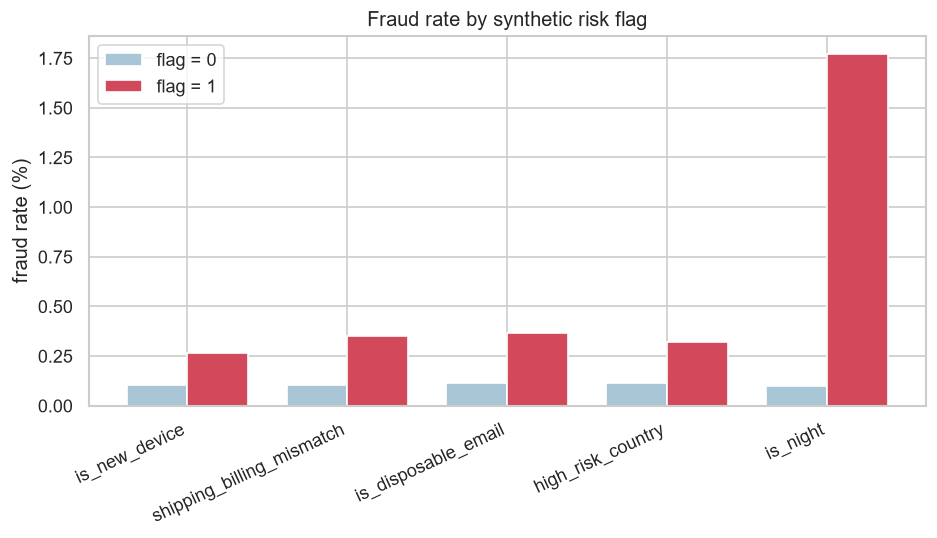
\includegraphics[width=\textwidth]{figures/06_synthetic_risk_flags.png}
\captionof{figure}{Fraud rate by synthetic risk flag.}
\label{fig:flags}
\end{minipage}\hfill
\begin{minipage}{0.42\textwidth}
\centering
\small
\begin{tabular}{@{}lrr@{}}
\toprule
\textbf{Signal} & \textbf{if 0 \%} & \textbf{if 1 \%}\\
\midrule
\code{is\_new\_device} & 0.102 & 0.268\\
\code{shipping\_billing\_mismatch} & 0.106 & 0.353\\
\code{is\_disposable\_email} & 0.116 & 0.365\\
\code{high\_risk\_country} & 0.114 & 0.320\\
\code{is\_night} & 0.100 & 1.773\\
\bottomrule
\end{tabular}
\captionof{table}{Fraud rate by flag value.}
\label{tab:flags}
\end{minipage}

\vspace{0.3cm}
Numeric context fields tell the same story (Figure~\ref{fig:numeric}): fraudulent accounts
are younger, sit farther from their billing IP, and have more failed payment attempts - but
the distributions overlap heavily, so no single field is a silver bullet.

\begin{figure}[h]
\centering

\includegraphics[width=0.92\textwidth]{figures/07_numeric_context_by_class.png}
\caption{Numeric context by class: account age, IP–billing distance, failed attempts.}
\label{fig:numeric}
\end{figure}

\section{Balance signature - an early leakage warning}
\label{sec:balance}

PaySim's balance-reconciliation fields are \emph{extraordinarily} predictive
(Figure~\ref{fig:balance}). The origin balance error and the ``account drained'' flag alone
achieve directionless AUCs of 0.92 and 0.87 (Table~\ref{tab:balancesig}). In particular,
97.6\% of frauds drain the origin account (\code{orig\_drained}) versus 23.8\% of
legitimate transactions.

\begin{warnbox}
\textbf{Leakage warning.} These signals are computed from the balance \emph{after} the
transaction settles, which is unknown at authorization time. A model that leans on them
looks near-perfect offline but cannot be deployed. We therefore split features into a
\emph{leaky} reference track and a \emph{deployable} authorization-time track
(Chapter~\ref{ch:m4}) and ship only the latter.
\end{warnbox}

\begin{minipage}{0.55\textwidth}
\centering
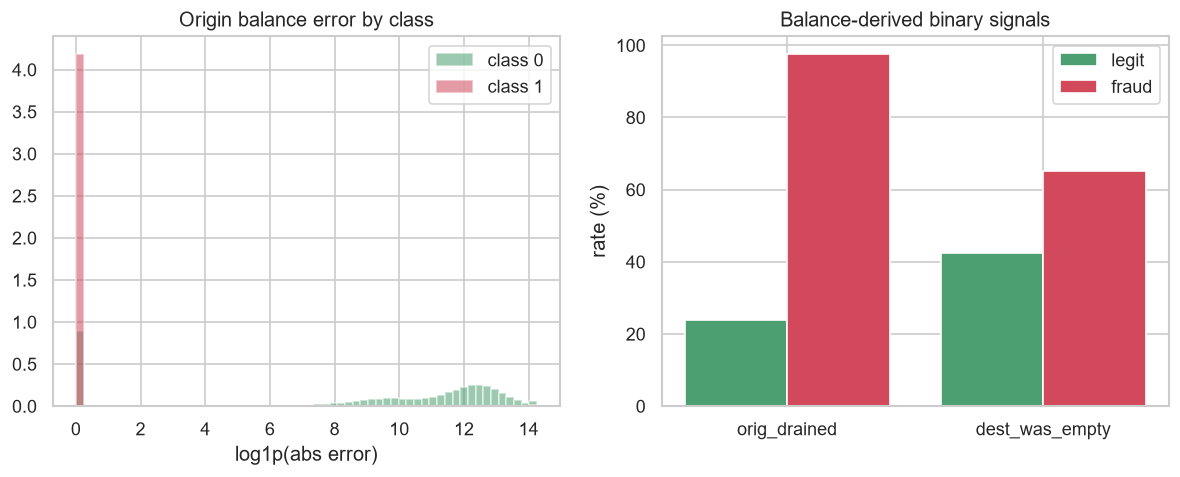
\includegraphics[width=\textwidth]{figures/08_balance_signature.png}
\captionof{figure}{Origin balance error and balance-derived flags by class.}
\label{fig:balance}
\end{minipage}\hfill
\begin{minipage}{0.42\textwidth}
\centering
\small
\begin{tabular}{@{}lr@{}}
\toprule
\textbf{Feature} & \textbf{Dir.less AUC}\\
\midrule
\code{abs\_errorBalanceOrig} & 0.921\\
\code{orig\_drained} & 0.869\\
\code{dest\_was\_empty} & 0.613\\
\code{abs\_errorBalanceDest} & 0.548\\
\bottomrule
\end{tabular}
\captionof{table}{Single-feature discriminative power of balance signals.}
\label{tab:balancesig}
\end{minipage}

\section{Destination reuse and the mule pattern}

Although origin accounts are single-use, \emph{destination} accounts are frequently reused:
2{,}722{,}362 unique destinations, of which 459{,}658 receive $\ge$2 transactions and one
receives 113. Crucially, the fraud rate rises monotonically with reuse
(Figure~\ref{fig:destreuse}, Table~\ref{tab:destreuse}): destinations seen 11+ times have a
1.69\% fraud rate versus 0.12\% for single-use destinations. This is the classic
\emph{mule-account} fan-in pattern and is the basis for our causal destination-history
features (Module 4).

\begin{minipage}{0.55\textwidth}
\centering

\includegraphics[width=\textwidth]{figures/09_destination_reuse_pattern.png}
\captionof{figure}{Destination reuse and fraud rate by reuse bucket.}
\label{fig:destreuse}
\end{minipage}\hfill
\begin{minipage}{0.42\textwidth}
\centering
\small
\begin{tabular}{@{}lrr@{}}
\toprule
\textbf{Reuse} & \textbf{Dests} & \textbf{Fraud \%}\\
\midrule
1 & 2{,}262{,}704 & 0.118\\
2–3 & 134{,}343 & 0.938\\
4–10 & 195{,}029 & 1.041\\
11+ & 130{,}286 & 1.692\\
\bottomrule
\end{tabular}
\captionof{table}{Fraud-destination rate by reuse bucket.}
\label{tab:destreuse}
\end{minipage}

\section{Channels and correlations}

Browser and OS carry essentially no fraud signal (rates flat at $\approx$0.12–0.13\%), as
expected from uniform synthetic generation. Billing country does carry signal - the
high-risk countries NG/ID/CN/RU top the chart at $\approx$0.32\%
(Figure~\ref{fig:channels}). Finally, linear correlations with the target
(Figure~\ref{fig:corr}) are all individually weak ($|r|<0.08$): \code{amount},
\code{orig\_drained}, \code{is\_night}, \code{errorBalanceDest}, and \code{isFlaggedFraud}
lead. The weakness of \emph{linear} correlations, contrasted with the strong tree-model
results later, is itself evidence that fraud here is a non-linear, interaction-driven
phenomenon.

\begin{figure}[h]
\centering
\begin{subfigure}{0.62\textwidth}
  
\includegraphics[width=\textwidth]{figures/10_context_channels.png}
  \caption{Fraud rate by browser, OS, and billing country.}
  \label{fig:channels}
\end{subfigure}\hfill
\begin{subfigure}{0.36\textwidth}
  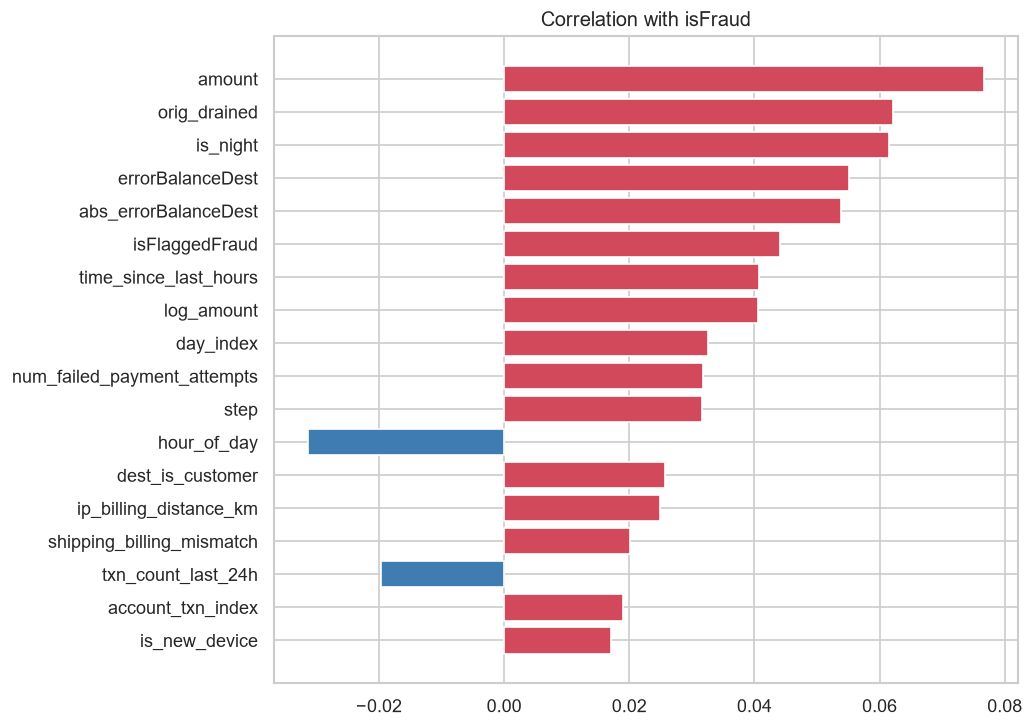
\includegraphics[width=\textwidth]{figures/11_corr_with_target.png}
  \caption{Top Pearson correlations with \code{isFraud}.}
  \label{fig:corr}
\end{subfigure}
\caption{Channel context and linear correlations with the target.}
\end{figure}

\begin{keybox}
\textbf{EDA takeaways.} (1) Extreme imbalance $\Rightarrow$ AUC-PR + cost-based threshold.
(2) Fraud lives only in TRANSFER/CASH\_OUT, at night, in large amounts.
(3) Balance fields are leaky $\Rightarrow$ deployable-vs-reference split.
(4) Destination reuse is a real, causal mule signal.
(5) Signals are individually weak and overlapping $\Rightarrow$ a non-linear model is needed.
\end{keybox}

%==============================================================================
\chapter{Data Cleaning (Module 3)}
\label{ch:m3}
%==============================================================================

\section{Philosophy: validate, document, preserve}

PaySim is a clean simulation, so aggressive cleaning would destroy signal rather than add
value. Our policy (\code{src/cleaning.py}) is deliberately conservative: \emph{validate and
document} everything, but \emph{remove} only exact duplicates or negative amounts, and
\emph{preserve} the balance-reconciliation quirks because they are predictive (their
leakage risk is handled at the feature stage, not by deletion).

\section{Findings and decisions}

\begin{itemize}[nosep,leftmargin=1.4em]
  \item \textbf{Missing values:} none in any of the 33 input columns.
  \item \textbf{Duplicates:} 0 exact duplicates on the PaySim base columns.
  \item \textbf{Negative amounts:} 0. \textbf{Steps outside 1..743:} 0.
  \item \textbf{Zero-amount rows:} 16 found - kept and marked with a new
        \code{flag\_zero\_amount} column rather than dropped.
  \item \textbf{Category validation:} \code{type}, \code{browser}, \code{device\_os},
        \code{billing\_country} all match their expected value sets exactly; no
        normalization needed.
  \item \textbf{Outliers:} amounts above the 99.9th percentile (6{,}363 rows) are kept but
        an optional \code{amount\_capped} column (winsorised at p99.9) is added for robust
        modelling.
  \item \textbf{Balance quirks preserved:} 2.32M rows with zero destination balances
        before/after, and millions of reconciliation ``errors'', are retained as signal.
\end{itemize}

Table~\ref{tab:cleanba} gives the before/after summary. Net effect: two audit columns added,
zero rows removed - a fully documented, reversible cleaning step.

\begin{table}[h]
\centering
\small
\begin{tabular}{@{}lrrr@{}}
\toprule
\textbf{Metric} & \textbf{Before} & \textbf{After} & \textbf{Change}\\
\midrule
Rows & 6{,}362{,}620 & 6{,}362{,}620 & 0\\
Columns & 33 & 35 & $+2$\\
Fraud rows & 8{,}213 & 8{,}213 & 0\\
Fraud rate & 0.129\% & 0.129\% & 0\\
Missing cells & 0 & 0 & 0\\
Duplicate base rows & 0 & 0 & 0\\
Negative amounts & 0 & 0 & 0\\
Zero-amount rows & 16 & 16 (flagged) & 0\\
\bottomrule
\end{tabular}
\caption{Cleaning before/after summary. Two columns added
(\code{flag\_zero\_amount}, \code{amount\_capped}); no rows removed.}
\label{tab:cleanba}
\end{table}

%==============================================================================
\chapter{Feature Engineering and Imbalance Handling (Module 4)}
\label{ch:m4}
%==============================================================================

\section{The authorization-time principle}

The overriding design rule is \textbf{causality}: a feature may use only information
available at the moment the transaction is authorized. This rules out post-transaction
balances and any aggregate that peeks at future rows. Getting this wrong is the most common
way fraud models fail in production, so we enforce it structurally, not just by convention.

\section{Chronological split (no test peeking)}

We split \emph{by time} on \code{step} (Table~\ref{tab:split}), not randomly, so training
always precedes validation/test - a realistic ``predict the future'' setup that also
surfaces temporal drift.

\begin{table}[h]
\centering
\small
\begin{tabular}{@{}lrrl@{}}
\toprule
\textbf{Split} & \textbf{Rows} & \textbf{Fraud rate} & \textbf{Step window}\\
\midrule
Train & 4{,}453{,}834 & 0.0818\% & 1–323\\
Validation & 954{,}393 & 0.0589\% & 323–378\\
Test & 954{,}393 & 0.4200\% & 378–743\\
\bottomrule
\end{tabular}
\caption{Time-based 70/15/15 split. The higher test fraud rate reflects genuine temporal
non-stationarity - a useful stress test.}
\label{tab:split}
\end{table}

\section{Feature families}

Four families of features are engineered (\code{src/features.py}):

\begin{enumerate}[nosep,leftmargin=1.6em]
  \item \textbf{Base PaySim:} \code{amount}, \code{log\_amount}, \code{amount\_cents}
        (card-testing / round-number signal), pre-transaction balances, transfer/cash-out
        flags, and - in the reference track only - balance-reconciliation errors and
        drained/empty flags.
  \item \textbf{Destination history (causal, past-only):} 16 features aggregating each
        \code{nameDest}'s \emph{prior} behaviour - transaction count so far, amount
        sum/mean/std so far, unique senders so far (fan-in), per-type counts, recency
        (\code{time\_since\_dest\_last\_seen}), and anomaly ratios
        (\code{amount\_to\_dest\_mean\_ratio}, \code{amount\_dest\_zscore}). These are
        computed once on the full chronological frame \emph{before} splitting via cumulative
        sums, so validation/test rows inherit real training-era history but never see the
        future.
  \item \textbf{Synthetic / context:} the Module-1 risk signals plus derived time features
        and illustrative velocity.
  \item \textbf{Categorical encodings:} fixed one-hot for \code{type}; train-frequency
        encoding for \code{browser}, \code{device\_os}, \code{billing\_country}. Raw
        IDs/display fields (\code{nameOrig}, \code{nameDest}, \code{customer\_id},
        \code{email}, \dots) are dropped from the model matrix.
\end{enumerate}

\section{Feature groups: leaky vs.\ deployable}

To quantify the cost of avoiding leakage, features are organised into five overlapping
groups (Table~\ref{tab:groups}). The two groups containing post-transaction balances are
marked \emph{leaky} and serve only as an upper-bound reference; the deployed model is chosen
from the deployable groups.

\begin{table}[h]
\centering
\small
\begin{tabularx}{\textwidth}{@{}l r l Y@{}}
\toprule
\textbf{Group} & \textbf{\#feat.} & \textbf{Status} & \textbf{Contents}\\
\midrule
\code{base} & 18 & \textcolor{brandaccent}{\bfseries leaky} & Full PaySim amount/balance signature (incl.\ post-txn balances).\\
\code{dest} & 16 & \textcolor{brandteal}{\bfseries deployable} & Past-only destination-account behaviour.\\
\code{synth} & 21 & \textcolor{brandteal}{\bfseries deployable} & Synthetic/contextual risk + encoded categoricals.\\
\code{realistic} & 44 & \textcolor{brandteal}{\bfseries deployable} & Authorization-time base + destination history + context. \textbf{(deployed)}\\
\code{all} & 50 & \textcolor{brandaccent}{\bfseries leaky} & Everything (base + dest + synth + encodings).\\
\bottomrule
\end{tabularx}
\caption{Feature groups. \code{realistic} is the deployable superset and drives the saved
bundle; \code{base}/\code{all} include leaky balance fields and are reference-only.}
\label{tab:groups}
\end{table}

\section{Leakage-aware transformer}

A single \code{FeatureTransformer} object encapsulates all state that must be
\emph{train-fitted}: the frequency-encoding maps, a median imputer, and a
\code{StandardScaler} (for the linear model). It exposes two matrices - a \code{tree}
matrix (raw, NaN-tolerant) for XGBoost/Random Forest and a \code{linear} matrix (imputed +
scaled) for Logistic Regression. Validation/test data are only ever \emph{transformed} with
train-fitted state, eliminating train/serve skew. The transformer even refuses to run on raw
subsets that lack precomputed destination history, turning the causality rule into an
enforced invariant.

\subsection{Automated leakage checks}

Four assertions run on every build (Table~\ref{tab:leakcheck}); all pass. These guard the
two most dangerous mistakes: a destination's first-ever transaction leaking a non-zero
history, and raw identifiers slipping into the matrix.

\begin{table}[h]
\centering
\small
\begin{tabularx}{\textwidth}{@{}Y c@{}}
\toprule
\textbf{Check} & \textbf{Status}\\
\midrule
First transaction to each destination has \code{dest\_txn\_count\_so\_far}$=0$ & PASS\\
\code{time\_since\_dest\_last\_seen}$=-1$ for unseen destinations & PASS\\
Raw display/ID columns absent from the feature matrix & PASS\\
Transformer rejects raw subsets lacking precomputed destination history & PASS\\
\bottomrule
\end{tabularx}
\caption{Automated leakage checks (all pass).}
\label{tab:leakcheck}
\end{table}

\section{Handling severe class imbalance}

With a train fraud rate of 0.0818\%, the negative:positive ratio is $\approx$1{,}221:1. We
address this through:

\begin{itemize}[nosep,leftmargin=1.4em]
  \item \textbf{Cost-sensitive learning (default):} \code{class\_weight="balanced"} for
        Logistic Regression and Random Forest, and \code{scale\_pos\_weight}$\,\approx1{,}221.57$
        for XGBoost. This re-weights the minority class without discarding or fabricating
        data.
  \item \textbf{Resampling (optional, train-fold only):} \code{src/imbalance.py} provides
        SMOTE and random undersampling, applied \emph{strictly inside the training fold
        after transformation} - validation/test folds are never resampled, so evaluation
        stays honest.
  \item \textbf{Metric choice:} evaluation uses AUC-PR and the cost function, which remain
        informative under imbalance where accuracy and ROC-AUC can be misleadingly high.
\end{itemize}

Constant columns are dropped on train (0 in this build). The final matrices carry 50 tree
features / 50 linear features, of which 16 are destination-history and 8 are encoded
categoricals.

%==============================================================================
\chapter{Model Development and Evaluation (Module 5)}
\label{ch:m5}
%==============================================================================

\section{Methodology}

Model development (\code{src/train\_validate.py}) follows a disciplined protocol designed to
prevent optimistic bias:

\begin{enumerate}[nosep,leftmargin=1.6em]
  \item \code{prepare\_feature\_frame} runs \emph{once} before splitting so causal
        destination history is consistent across folds.
  \item Every (model $\times$ feature-group) pair is trained on \code{train}.
  \item The \textbf{operating threshold} is chosen on \code{validation} by minimising the
        expected cost of Eq.~\eqref{eq:cost}.
  \item The \textbf{best deployable configuration} is chosen on \code{validation} cost -
        never on test.
  \item \code{test} is evaluated \textbf{exactly once} for the selected configuration.
  \item Leaky groups (\code{base}, \code{all}) are \emph{excluded from bundle selection};
        they remain in the comparison table only as an upper-bound reference.
\end{enumerate}

\section{Candidate models}

Three families required by the brief are compared (Table~\ref{tab:hparams}). XGBoost is a
gradient-boosted tree ensemble expected to excel on the non-linear, interaction-heavy signal
the EDA revealed; Random Forest is a bagged-tree baseline; Logistic Regression is a linear
baseline that also stress-tests whether the problem is linearly separable (the EDA suggested
not).

\begin{table}[h]
\centering
\small
\begin{tabularx}{\textwidth}{@{}l l Y@{}}
\toprule
\textbf{Model} & \textbf{Matrix} & \textbf{Key hyperparameters}\\
\midrule
Logistic Regression & linear & \code{max\_iter=1000}, \code{class\_weight=balanced}\\
Random Forest & tree & \code{n\_estimators=120}, \code{min\_samples\_leaf=2}, \code{class\_weight=balanced\_subsample}\\
XGBoost & tree & \code{n\_estimators=220}, \code{max\_depth=5}, \code{learning\_rate=0.08}, \code{subsample=0.9}, \code{colsample\_bytree=0.9}, \code{scale\_pos\_weight}$\approx$1221, \code{eval\_metric=aucpr}\\
\bottomrule
\end{tabularx}
\caption{Model families and hyperparameters.}
\label{tab:hparams}
\end{table}

\section{Evaluation metrics for imbalanced data}

We report metrics suited to a 0.13\%-prevalence problem: \textbf{AUC-PR} (primary - the
area under the precision–recall curve, which unlike ROC-AUC is sensitive to the minority
class), \textbf{ROC-AUC}, \textbf{precision / recall / F1} at the operating point, the
\textbf{expected cost} of Eq.~\eqref{eq:cost}, and \textbf{loss avoided \%} (share of
fraudulent money intercepted).

\section{Cost-based threshold selection}
\label{sec:cost}

The threshold is not fixed at 0.5; it is swept over a grid and the value minimising
validation expected cost is chosen. The three cost coefficients are derived rather than
guessed (methodology in \code{docs/cost\_model\_worksheet.md}); the values currently in
\code{src/config.py} are:

\begin{table}[h]
\centering
\small
\begin{tabularx}{\textwidth}{@{}l l Y@{}}
\toprule
\textbf{Coefficient} & \textbf{Value} & \textbf{Rationale}\\
\midrule
$c_{FN}$ (missed fraud) & $1.0 \times$ amount & Push-payment fraud has near-zero recovery; we lose $\approx$100\% of the amount.\\
$c_{FP}$ (false alarm) & 25.0 / case & Lost margin $+$ churn risk $+$ support cost for a wrongly blocked customer.\\
$c_{MR}$ (manual review) & 3.0 / case & Fully-loaded analyst labour per reviewed transaction.\\
\bottomrule
\end{tabularx}
\caption{Business-cost coefficients (assumptions; see the cost-model worksheet for the
sourcing method).}
\label{tab:costcoef}
\end{table}

\subsection{Break-even and why the model blocks widely}

Only the \emph{ratio} of coefficients matters. The break-even amount - the fraud value at
which blocking is worthwhile even at the risk of a false positive - is
\[
\text{break-even} = \frac{c_{FP}}{c_{FN}} = \frac{25}{1} = 25 \text{ currency units}.
\]
Because the median fraudulent amount in PaySim is enormous (hundreds of thousands),
essentially \emph{every} suspected fraud is worth blocking. The rational consequence is an
operating point with \textbf{very high recall and modest precision}: the model deliberately
casts a wide net because a missed large-value fraud costs far more than a review. This is a
correct, intended outcome of the cost model, not a defect - and it is why we report loss
avoided and flagged-rate alongside precision.

\begin{keybox}
\textbf{Recommended next step (sensitivity analysis).} Because the coefficients are
assumptions, the report should sweep $c_{FP}\in\{10,25,50,100,200\}$, re-select the
threshold each time, and show that the operating point (recall, precision, flagged rate) is
stable across a plausible range. A helper (\code{src/cost\_sensitivity.py}) is proposed for
Module 8.
\end{keybox}

\section{Results}

\subsection{Deployable model comparison (\code{realistic} group)}

Table~\ref{tab:realistic} compares the three models on the deployable \code{realistic}
group. \textbf{XGBoost} is the clear winner on every axis that matters: the highest test
AUC-PR (0.907) and F1 (0.294), while still catching 98.1\% of fraud and avoiding 99.9\% of
loss. Logistic Regression confirms the EDA's hint - a linear model cannot separate this data
(test AUC-PR 0.587) and compensates with an untenable flag rate. Random Forest is
competitive but trails XGBoost.

\begin{table}[h]
\centering
\small
\begin{tabular}{@{}l rrrrrr@{}}
\toprule
\textbf{Model (realistic)} & \textbf{AUC-PR} & \textbf{ROC-AUC} & \textbf{Precision} & \textbf{Recall} & \textbf{F1} & \textbf{Loss avd.}\\
\midrule
\textbf{XGBoost} & \textbf{0.907} & 0.999 & 0.173 & 0.981 & \textbf{0.294} & 99.91\%\\
Random Forest & 0.812 & 0.974 & 0.084 & 0.953 & 0.155 & 99.60\%\\
Logistic Regression & 0.587 & 0.990 & 0.025 & 0.997 & 0.049 & 99.98\%\\
\bottomrule
\end{tabular}
\caption{Held-out \emph{test} metrics on the deployable \code{realistic} group (threshold
selected on validation). XGBoost is selected for deployment.}
\label{tab:realistic}
\end{table}

\subsection{Feature-group ablation (XGBoost)}

Holding the model fixed at XGBoost and varying the feature group
(Table~\ref{tab:ablation}) makes the leakage story concrete. The leaky groups
(\code{base}, \code{all}) reach an artificial test AUC-PR of $\approx$1.0 - driven entirely
by the post-transaction balance fields. Among deployable groups, neither destination history
alone (\code{dest}) nor context alone (\code{synth}) is sufficient; only their combination
in \code{realistic} yields strong, honest performance (0.907). This is the core empirical
justification for the deployed feature set.

\begin{table}[h]
\centering
\small
\begin{tabular}{@{}l c rrrr@{}}
\toprule
\textbf{Group} & \textbf{Leaky?} & \textbf{\#feat.} & \textbf{Test AUC-PR} & \textbf{Test recall} & \textbf{Loss avd.}\\
\midrule
\code{base} & yes & 18 & 1.000$^{\dagger}$ & 0.9995 & 99.99\%\\
\code{all}  & yes & 50 & 1.000$^{\dagger}$ & 0.9995 & 99.99\%\\
\code{realistic} & no & 44 & \textbf{0.907} & 0.981 & 99.91\%\\
\code{synth} & no & 21 & 0.243 & 0.961 & 96.21\%\\
\code{dest}  & no & 16 & 0.009 & 0.998 & 99.77\%\\
\bottomrule
\end{tabular}
\caption{XGBoost across feature groups. $^{\dagger}$Leaky groups are an upper-bound
reference only - \emph{not} deployable. The deployable optimum is \code{realistic}.}
\label{tab:ablation}
\end{table}

\subsection{Selected model - the deployed configuration}

The saved bundle (\code{models/fraud\_model.joblib}) is \textbf{XGBoost on \code{realistic}
(44 features)} with a validation-selected threshold of \textbf{0.241}. Its full profile is
in Table~\ref{tab:deployed}. The validation$\to$test AUC-PR change (0.806$\to$0.907) is
favourable and consistent with the higher, more separable fraud regime in the later test
window; ROC-AUC is essentially identical across folds (0.999), indicating stable ranking.

\begin{table}[h]
\centering
\small
\begin{tabular}{@{}l rr@{}}
\toprule
\textbf{Metric} & \textbf{Validation} & \textbf{Test}\\
\midrule
AUC-PR & 0.806 & 0.907\\
ROC-AUC & 0.9990 & 0.9987\\
Operating threshold & \multicolumn{2}{c}{0.241 (selected on validation)}\\
Precision & 0.029 & 0.173\\
Recall & 0.989 & 0.981\\
F1 & 0.056 & 0.294\\
Flagged rate & 2.03\% & 2.38\%\\
Loss avoided & 99.98\% & 99.91\%\\
\bottomrule
\end{tabular}
\caption{Deployed model: XGBoost / \code{realistic} / 44 features / threshold 0.241.}
\label{tab:deployed}
\end{table}

\subsection{Interpreting the operating point}

At the chosen threshold on the test window the model flags 2.38\% of all transactions,
catches 98.1\% of frauds, and intercepts 99.9\% of the fraudulent money. Precision is 17\%
by design (Section~\ref{sec:cost}): roughly five of every six flags are false alarms sent to
review, which the cost model accepts because the alternative - missing a six-figure fraud -
is far costlier. Two thresholds are exposed downstream (Module 6): the review threshold
(0.241) and a high-confidence auto-block threshold, enabling an \emph{allow / review / block}
policy rather than a binary decision.

\begin{warnbox}
\textbf{Honesty note.} We deliberately do \emph{not} headline the AUC-PR$\approx$1.0
achievable with balance features. Those numbers are real but non-deployable; reporting them
as the result would be misleading. The deployable 0.907 is the number the business can
actually rely on at authorization time.
\end{warnbox}

\section{From a single model to a deployed three-model ensemble}
\label{sec:ensemble}

Rather than ship one classifier, the serving layer packages \emph{all three} models trained
on the deployable \code{realistic} group into a single bundle,
\code{models/fraud\_ensemble.joblib} (built by \code{src/train\_validate.py}, consumed
through \code{src/ensemble.py}). The bundle stores one shared \code{FeatureTransformer} plus,
per model, its fitted estimator, feature matrix (\code{tree}/\code{linear}), feature list,
and \emph{own} cost-tuned decision threshold. The single best model
(\code{fraud\_model.joblib}) is retained separately for batch scoring
(\code{src/infer.py}).

At scoring time every model votes independently and the verdicts are combined by a
\textbf{max-risk} rule - the most severe decision wins (\code{block > review > allow}) - with
per-model thresholds and a shared high-confidence block floor of \textbf{0.9}
(Eq.~\ref{eq:decide}):
\begin{equation}
\label{eq:decide}
\text{decide}(p, \tau) =
\begin{cases}
\text{block} & p \ge \max(0.9,\ \tau)\\
\text{review} & \tau \le p < \max(0.9,\ \tau)\\
\text{allow} & p < \tau
\end{cases}
\qquad
\text{aggregate} = \max_{\text{severity}} \{\text{decide}(p_m,\tau_m)\}_m .
\end{equation}
This design buys two things over a single model: (i) a max-risk \emph{union} raises recall
(any model can escalate a suspicious case), matching the cost model's preference for catching
fraud; and (ii) \textbf{graceful degradation} - if one model errors at request time, its
entry is dropped, the aggregate is computed from the survivors, and the response is flagged
\code{degraded} rather than failing. The same \code{src/ensemble.py} scoring path backs both
the API (single record, via \code{score\_record}) and the Streamlit batch (via
\code{score\_batch}), so a transaction gets an identical verdict either way - train/serve
parity by construction.

\begin{keybox}
\textbf{Reproducibility note.} All results in this chapter are the \textbf{full-data
(6.36M-row)} build, and the deployed app (Chapter~\ref{ch:m6}) scores on that same build.
The trained ensemble bundle ($\approx$60\,MB) is committed to git so the app works
immediately after clone, but the processed feature dataset ($\approx$526\,MB on full PaySim)
exceeds GitHub's 100\,MB limit and is regenerated locally by the data pipeline; a committed
$\approx$26\,MB stratified sample (\code{context\_sample.parquet}) lets a fresh clone run the
app in \emph{sample mode} without the full rebuild.
\end{keybox}

%==============================================================================
\chapter{Deployment (Module 6)}
\label{ch:m6}
%==============================================================================

The deployable model of Chapter~\ref{ch:m5} is packaged into a working analytics product:
a real-time scoring API and an eight-page analyst application, engineered to run on a single
free-tier cloud port. All money figures across the API, the app, and this report come from
one shared cost module (\code{src/costs.py}), so the three can never disagree on what a
decision is worth.

\section{Real-time scoring API}

A FastAPI service (\code{api/main.py}) loads the ensemble bundle at start-up and exposes two
endpoints. \code{GET /} is a health check listing the loaded models and the aggregate rule.
\code{POST /score} accepts a transaction payload and, following the flow in
Section~\ref{sec:ensemble}, enriches the single record (destination-history features disabled
because a live request has no prior context), scores it with all three models, and returns
each model's probability and \emph{allow / review / block} decision plus the max-risk
aggregate verdict. A per-model failure is isolated: that model returns an \code{error} entry,
the aggregate falls back to the survivors, and the response is marked \code{degraded}.

\begin{figure}[h]
\centering
\begin{minipage}{0.95\textwidth}
{\footnotesize
\begin{verbatim}
POST /score   ->   HTTP 200
{
  "models": {
    "logreg": {"model_name": "Logistic Regression",
               "fraud_probability": 0.63, "decision": "review",
               "review_threshold": 0.52, "block_threshold": 0.90},
    "rf":     {"model_name": "Random Forest",
               "fraud_probability": 0.95, "decision": "block", ...},
    "xgb":    {"model_name": "XGBoost",
               "fraud_probability": 0.88, "decision": "review", ...}
  },
  "aggregate": {"decision": "block", "rule": "max-risk"}
}
\end{verbatim}
}
\end{minipage}
\caption{Example \code{POST /score} response: three independent verdicts plus the max-risk
aggregate. Here Random Forest escalates to \emph{block}, so the aggregate blocks.}
\label{fig:apiresp}
\end{figure}

\section{Transparent reason codes}

For every flagged transaction the review queue shows a short, human-readable list of
\emph{why} it was flagged (\code{src/reasons.py}). We deliberately use rule-based reason
codes - e.g. ``2 failed payment attempts'', ``high-risk country'', ``IP 1{,}300\,km from
billing'', ``account fully drained'', ``shipping $\ne$ billing'', ``new account (12d)'' -
rather than a black-box attribution such as SHAP: for a fraud analyst, and for a regulator,
a concrete list of the risk signals actually present is more actionable and more defensible
than a bar chart of feature weights. The reason codes \emph{explain}; the ensemble score
still \emph{decides}.

\section{Shared cost / ROI model}

\code{src/costs.py} turns any decision vector plus ground-truth labels and amounts into a
full money breakdown using the Section~\ref{sec:cost} coefficients: fraud exposure, caught
vs.\ missed amount, false-positive cost, review labour, and the resulting \emph{net savings}
versus two baselines (do-nothing and review-everything), plus an ROI figure (savings per unit
of operating spend). The Cost \& ROI page lets an analyst edit the cost matrix live and see
the cost-optimal threshold move - making the fraud/friction trade-off tangible in currency
rather than abstract metrics.

\section{Eight-page analyst application}

A multi-page Streamlit application (\code{app/streamlit\_app.py} via \code{st.navigation})
presents the product as a capstone narrative - pitch $\to$ problem $\to$ product $\to$ rigour
$\to$ value $\to$ real-time $\to$ operations $\to$ serving (Table~\ref{tab:pages}). Every
analytical page carries a data-provenance badge, and model metrics are always reported on the
held-out temporal test split.

\begin{table}[h]
\centering
\small
\begin{tabularx}{\textwidth}{@{}l Y l@{}}
\toprule
\textbf{Page} & \textbf{What it shows} & \textbf{Data}\\
\midrule
Overview & Executive KPIs: money saved, fraud loss avoided, recall/precision, model health & test\\
Segment Analytics & Where fraud concentrates: by type, hour, amount + risk-factor lift & full population\\
Review Queue & Triage with per-transaction reason codes; 3 models + max-risk verdict & 2k sample\\
Model Evaluation & AUC-PR / ROC / PR curves, confusion matrix, cumulative-gains / lift & test\\
Cost \& ROI & Prices the trade-off in money terms; per-model vs.\ ensemble; editable cost matrix & test\\
Live Feed & Simulated real-time scoring stream & simulated\\
Monitoring & PSI drift detection $\to$ retraining + alerting (Chapter~\ref{ch:m7}) & simulated\\
API Tester & Score a hand-built transaction through the live \code{/score} endpoint & live API\\
\bottomrule
\end{tabularx}
\caption{The eight pages of the Streamlit analyst application.}
\label{tab:pages}
\end{table}

\section{Single-port cloud deployment}

Free hosts such as Streamlit Community Cloud and Hugging Face Spaces expose only one public
port. To keep the live API Tester working without a second port,
\code{app/embedded\_api.py} launches the FastAPI service in a background thread on
\code{127.0.0.1:8000} inside the container; the app calls it \emph{server-side} over
localhost, so the browser only ever talks to Streamlit (and if a local \code{uvicorn} is
already running, the open port is detected and reused). Deployment then reduces to: commit the
runtime artefacts (the $\approx$60\,MB ensemble bundle and the preview CSV, kept in git via
\code{.gitignore} exceptions; the $\approx$526\,MB processed dataset exceeds GitHub's limit and
is rebuilt locally, with a committed $\approx$26\,MB stratified sample as a fresh-clone fallback),
point Streamlit Cloud at
\code{app/streamlit\_app.py}, and let \code{requirements.txt} and \code{packages.txt}
(\code{libgomp1} for XGBoost) install automatically.

\begin{todobox}
\textbf{Remaining for submission.} Publish the app to a free tier and paste the resulting
\textbf{live link} here (a graded deliverable), together with one or two screenshots of the
review queue and monitoring pages.
\end{todobox}

%==============================================================================
\chapter{Monitoring (Module 7)}
\label{ch:m7}
%==============================================================================

A deployed fraud model decays as fraud tactics and customer behaviour shift. Module 7 closes
the loop with a monitoring layer that detects distribution drift, decides when to retrain,
performs the retraining, and raises an alert - all surfaced on the Monitoring page of the
analyst app.

\section{Drift detection with the Population Stability Index}

\code{monitoring/drift.py} quantifies drift with the \textbf{Population Stability Index
(PSI)}, comparing a reference window (earlier half of the stream, by \code{day\_index}) to a
current window (later half):
\begin{equation}
\text{PSI} = \sum_{b} \big(c_b - r_b\big)\,\ln\!\frac{c_b}{r_b},
\end{equation}
where $r_b, c_b$ are the reference/current fractions in bin $b$ (reference-quantile bins).
PSI is transparent and dependency-free. We use the industry-standard bands
$\text{PSI}<0.10$ (stable), $0.10$–$0.25$ (moderate - monitor), and $>0.25$ (significant).
Critically, PSI is computed both on the \textbf{input features} (\code{amount},
\code{account\_age\_days}, \code{ip\_billing\_distance\_km}, failed attempts, new-device,
hour) \emph{and} on each model's \textbf{predicted-score distribution}
(\code{PREDICTION\_SCORE\_logreg/\_rf/\_xgb}) - so both data drift and per-model concept
drift are visible.

\section{Retraining trigger and self-validation}

A \textbf{retraining trigger} fires when any monitored PSI reaches \textbf{0.25}. The module
validates its own detector: alongside the natural earlier-vs-later split it constructs a
\emph{simulated fraud campaign} (\code{inject\_drift}: amounts $\times1.25$–$1.6$, IP distance
$\times1.8$, extra failed attempts) and confirms the trigger stays quiet on the natural split
but fires on the injected one (Table~\ref{tab:drift}). This demonstrates the monitor catches
a real shift without false-alarming on benign temporal variation.

\begin{table}[h]
\centering
\small
\begin{tabular}{@{}l rl rl@{}}
\toprule
\textbf{Signal} & \multicolumn{2}{c}{\textbf{Natural split}} & \multicolumn{2}{c}{\textbf{Simulated campaign}}\\
 & PSI & band & PSI & band\\
\midrule
\code{amount} & low & stable & high & \textcolor{brandaccent}{\bfseries SIGNIFICANT}\\
\code{ip\_billing\_distance\_km} & low & stable & high & \textcolor{brandaccent}{\bfseries SIGNIFICANT}\\
\code{num\_failed\_payment\_attempts} & low & stable & elevated & moderate/SIG.\\
\code{PREDICTION\_SCORE\_*} (per model) & low & stable & elevated & moderate/SIG.\\
\bottomrule
\end{tabular}
\caption{Self-validating drift check: the natural split stays \emph{stable} while the injected
fraud campaign pushes feature and per-model prediction PSI past the 0.25 retraining trigger.}
\label{tab:drift}
\end{table}

\section{In-app retraining and alerting}

When the trigger fires, two operational responses are available:

\begin{itemize}[nosep,leftmargin=1.4em]
  \item \textbf{Retraining} (\code{src/retrain.py}): all three ensemble models are refit on a
        freshly generated, current-distribution labelled sample, \emph{reusing} the deployed
        transformer and each model's hyperparameters, and each decision threshold is
        re-selected by validation expected cost. This is a fast in-memory adaptation (seconds)
        for the live demo; the on-disk bundle is left untouched, so the operation is safe to
        trigger from the dashboard.
  \item \textbf{Alerting} (\code{src/alerting.py}): a Slack/Discord-compatible webhook payload
        and a downloadable Markdown incident report are generated, listing the signals that
        breached the threshold and their PSI values. Delivery uses only the standard library,
        never raises, and sends nothing unless a webhook URL is configured (kept out of git
        via \code{.streamlit/secrets.toml}).
\end{itemize}

\section{Monitoring dashboard}

The Monitoring page (\code{app/monitoring\_view.py}) has two tabs. \textbf{Reports} renders
the committed \code{drift\_report.md} and embeds the optional Evidently
(\code{DataDriftPreset}) HTML report. \textbf{Live} recomputes drift on demand: a
``simulate fraud campaign'' toggle applies \code{inject\_drift}, the PSI table (features plus
per-model prediction rows) is shown colour-banded, overlaid reference-vs-current histograms
explain each PSI value, and a retrain banner with the alert action appears when the trigger
fires.

\begin{todobox}
\textbf{Remaining for submission.} Capture the rendered Evidently dashboard and one
Monitoring-page screenshot for the appendix, and (optionally) add rolling-window
precision/recall as labels arrive, noting the label-delay caveat inherent to fraud feedback.
\end{todobox}

%==============================================================================
\chapter{Risk Policy, Limitations, and Future Work (Module 8)}
\label{ch:m8}
%==============================================================================

Modules 1–7 translate directly into an operating policy for the platform's risk team. Each
recommendation maps a signal to a concrete action - auto-block, manual review, or allow -
realised by the ensemble's max-risk thresholds and made auditable by the review queue's
reason codes.

\section{Risk-policy recommendations}

\begin{itemize}[nosep,leftmargin=1.4em]
  \item \textbf{Auto-block} only very-high-confidence cases (any model $\ge$ the 0.9 block
        floor), reserving hard friction for the clearest fraud.
  \item \textbf{Route to manual review} the mid-confidence band (between each model's
        cost-tuned review threshold and the block floor) - where the cost model already
        places most flags - and show the analyst the reason codes so the decision is
        explainable.
  \item \textbf{Prioritise} the review queue by \emph{expected loss} (risk score $\times$
        amount) so scarce analyst capacity chases the largest exposures first.
  \item \textbf{Apply cheap structural pre-filters:} only \code{TRANSFER}/\code{CASH\_OUT}
        can be fraud; a night-time, large-amount transfer to a frequently-reused destination
        warrants extra scrutiny even at a moderate score.
  \item \textbf{Escalate on drift:} when the Module-7 PSI trigger fires, retrain and alert
        before performance visibly degrades.
\end{itemize}

\begin{keybox}
\textbf{Which signals auto-block vs.\ review?} (the brief's core M8 question.) \emph{Auto-block}
is reserved for score-driven certainty (block floor) - no single raw signal auto-blocks,
because every synthetic signal overlaps between classes. \emph{Manual review} is triggered by
the mid-band score \emph{and} is where high-severity reason codes (multiple failed attempts,
high-risk country, drained account, large night-time transfer to a reused mule destination)
concentrate. \emph{Allow} covers the low-score majority. This keeps auto-block precise and
routes ambiguity to humans - matching the cost model's high-recall, review-heavy operating
point.
\end{keybox}

\section{Limitations}

\begin{itemize}[nosep,leftmargin=1.4em]
  \item PaySim is a simulation; its post-transaction balance dynamics are cleaner than
        reality - precisely why the leaky/deployable split (Chapters~\ref{ch:m4}--\ref{ch:m5})
        matters and why we never ship balance features.
  \item The contextual layer is synthetic; its parameters are plausible but not calibrated to
        a real platform, and real fraud would show richer cross-signal interactions.
  \item The cost coefficients are business assumptions; only their \emph{ratio} matters
        (Section~\ref{sec:cost}), and a sensitivity sweep is still recommended.
  \item Operating precision is low \emph{by design}; in production it is bounded by review
        capacity, an operational constraint that should be modelled explicitly.
  \item In-app retraining adapts on freshly generated, current-distribution data for the
        live demo; a production retrain would instead rely on real labelled feedback, which
        arrives with delay (chargeback / confirmation lag) and needs its own validation.
\end{itemize}

\section{Future work}

\begin{itemize}[nosep,leftmargin=1.4em]
  \item Publish the live link and add probability calibration (isotonic/Platt) so scores are
        interpretable as probabilities across models.
  \item A cost-coefficient sensitivity sweep and a capacity-constrained operating point.
  \item A full-data ensemble build plus explicit imbalance experiments (SMOTE vs.\
        undersampling vs.\ class weights).
  \item Graph features on the destination network for stronger mule detection, and a
        learned/weighted ensemble instead of the current max-risk union.
  \item Rolling-window performance monitoring (with label delay) and an automatically
        triggered - not just dashboard-initiated - retraining pipeline.
\end{itemize}

\section{Presentation and demo}

The deliverable is presented to the class through the live eight-page Streamlit application:
the narrative runs pitch $\to$ problem (Segment Analytics) $\to$ product (Review Queue)
$\to$ rigour (Model Evaluation) $\to$ value (Cost \& ROI) $\to$ real-time (Live Feed)
$\to$ operations (Monitoring) $\to$ serving (API Tester), mirroring the structure of this
report.

%==============================================================================
\chapter{Conclusion}
\label{ch:conclusion}
%==============================================================================

We built a reproducible, end-to-end fraud-detection product on PaySim augmented with a
documented synthetic risk layer, spanning the full eight-module lifecycle from raw data to a
monitored deployment. The project's distinctive contribution is methodological rigour under a
realistic constraint: by separating leaky post-transaction signals from deployable
authorization-time signals, we avoid the near-perfect-but-useless result that balance
features invite, and instead deliver a model the business can actually run. The reference
XGBoost model reaches a test AUC-PR of 0.907, recall of 98.1\%, and avoids 99.9\% of fraud
loss while flagging only 2.4\% of transactions - an operating point chosen not by accuracy
but by an explicit business cost function.

That model is productionised as a three-model max-risk ensemble behind a real-time scoring
API and an eight-page analyst application, deployable to a single free-tier port, and kept
honest by a PSI-based monitoring layer with a retraining trigger, in-app retraining, and
webhook alerting. The result is not just a classifier but a complete, auditable analytics
product: it scores transactions, explains its flags with reason codes, prices its decisions
in currency, and watches itself for drift - closing the loop the brief asks for. The one
remaining task is to publish the public live link and attach demo screenshots.

%==============================================================================
\appendix
\chapter{Appendix}
%==============================================================================

\section{Full model comparison}

Table~\ref{tab:fullresults} lists all fifteen (model $\times$ feature-group) configurations.
Leaky groups (\code{base}, \code{all}) are shaded conceptually as upper-bound references.

{\footnotesize
\setlength{\tabcolsep}{4.5pt}
\begin{longtable}{@{}l l c r rr rrr r@{}}
\caption{Full results - all models $\times$ feature groups (test metrics; threshold selected
on validation).}\label{tab:fullresults}\\
\toprule
\textbf{Model} & \textbf{Group} & \textbf{Leaky} & \textbf{\#f} & \textbf{val AUC-PR} & \textbf{test AUC-PR} & \textbf{Prec.} & \textbf{Recall} & \textbf{F1} & \textbf{Loss avd.}\\
\midrule
\endfirsthead
\toprule
\textbf{Model} & \textbf{Group} & \textbf{Leaky} & \textbf{\#f} & \textbf{val AUC-PR} & \textbf{test AUC-PR} & \textbf{Prec.} & \textbf{Recall} & \textbf{F1} & \textbf{Loss avd.}\\
\midrule
\endhead
\bottomrule
\endfoot
Logistic Reg. & base & yes & 18 & 0.523 & 0.774 & 0.119 & 0.992 & 0.213 & 98.85\%\\
Logistic Reg. & dest & no & 16 & 0.001 & 0.011 & 0.004 & 0.998 & 0.008 & 99.94\%\\
Logistic Reg. & synth & no & 21 & 0.065 & 0.217 & 0.010 & 1.000 & 0.020 & 100.0\%\\
Logistic Reg. & realistic & no & 44 & 0.249 & 0.587 & 0.025 & 0.997 & 0.049 & 99.98\%\\
Logistic Reg. & all & yes & 50 & 0.604 & 0.853 & 0.114 & 0.989 & 0.205 & 98.85\%\\
\midrule
Random Forest & base & yes & 18 & 1.000 & 1.000 & 1.000 & 0.9995 & 0.9998 & 99.99\%\\
Random Forest & dest & no & 16 & 0.001 & 0.006 & 0.006 & 0.803 & 0.012 & 85.54\%\\
Random Forest & synth & no & 21 & 0.289 & 0.138 & 0.030 & 0.751 & 0.058 & 75.55\%\\
Random Forest & realistic & no & 44 & 0.744 & 0.812 & 0.084 & 0.953 & 0.155 & 99.60\%\\
Random Forest & all & yes & 50 & 1.000 & 1.000 & 1.000 & 0.9995 & 0.9998 & 99.99\%\\
\midrule
XGBoost & base & yes & 18 & 1.000 & 1.000 & 1.000 & 0.9995 & 0.9998 & 99.99\%\\
XGBoost & dest & no & 16 & 0.001 & 0.009 & 0.004 & 0.998 & 0.008 & 99.77\%\\
XGBoost & synth & no & 21 & 0.268 & 0.243 & 0.011 & 0.961 & 0.022 & 96.21\%\\
\textbf{XGBoost} & \textbf{realistic} & \textbf{no} & \textbf{44} & \textbf{0.806} & \textbf{0.907} & \textbf{0.173} & \textbf{0.981} & \textbf{0.294} & \textbf{99.91\%}\\
XGBoost & all & yes & 50 & 1.000 & 1.000 & 1.000 & 0.9995 & 0.9998 & 99.99\%\\
\end{longtable}}

\section{Reproducibility}

\begin{itemize}[nosep,leftmargin=1.4em]
  \item Fixed seed \code{SEED=42} throughout; deterministic synthetic generation.
  \item Full rebuild: \code{./scripts/get\_data.sh} (Kaggle download) then
        \code{./train.sh full} runs Modules 1–5 on all 6.36M rows.
  \item Per-module entry points are listed in Table~\ref{tab:modmap}.
  \item Environment pinned in \code{requirements.txt} (pandas, scikit-learn, xgboost,
        imbalanced-learn, fastapi, streamlit, evidently).
\end{itemize}

\begin{thebibliography}{9}
\bibitem{paysim} E. A. Lopez-Rojas, A. Elmir, and S. Axelsson.
\emph{PaySim: A financial mobile money simulator for fraud detection.}
28th European Modeling and Simulation Symposium (EMSS), 2016.
\bibitem{kaggle} R. Roy. \emph{Online Payments Fraud Detection Dataset.} Kaggle.
\url{https://www.kaggle.com/datasets/rupakroy/online-payments-fraud-detection-dataset}
\bibitem{xgboost} T. Chen and C. Guestrin. \emph{XGBoost: A Scalable Tree Boosting System.}
KDD, 2016.
\bibitem{smote} N. V. Chawla et al. \emph{SMOTE: Synthetic Minority Over-sampling
Technique.} JAIR, 2002.
\bibitem{evidently} Evidently AI. \emph{Open-source ML monitoring.}
\url{https://www.evidentlyai.com/}
\end{thebibliography}

\end{document}
